\documentclass[]{amsart}

%\usepackage{times}
\usepackage{amssymb, mathrsfs, color, amsthm, tikz, subcaption, graphicx}
\usepackage[colorlinks=true, linkcolor=blue, citecolor=blue, urlcolor=blue]{hyperref}

%\usepackage[mathscr]{eucal}
%\usepackage[notref,notcite]{showkeys}

%\usepackage{tikz, pgfmath}
%\usepackage{fp}
%\usetikzlibrary {fixedpointarithmetic}
%\hoffset -1.2truecm \textwidth 5.8truein \textheight 8.5truein

\newtheorem{thm}{Theorem}[section]
\newtheorem{cor}[thm]{Corollary}
\newtheorem{lem}[thm]{Lemma}
\newtheorem{ex}[thm]{Example}
\newtheorem{prop}[thm]{Proposition}
\newtheorem{prob}[thm]{Problem}
\newtheorem{ques}[thm]{Question}
\newtheorem{rem}[thm]{Remark}
\newtheorem{thmx}{Theorem}


\numberwithin{equation}{section}

%%%%%%% Macros %%%%%%%%%%%
\renewcommand{\phi}{\varphi}

\renewcommand{\thethmx}{\Alph{thmx}}

%\newcommand{\bigoh}{\mbox{O}}

\newcommand{\cp}{C_\phi}

\newcommand{\R}{\mathbb{R}}

\newcommand{\N}{\mathbb{N}}

\newcommand{\F}{\mathbb{F}}

\newcommand{\D}{\mathbb{D}}

\newcommand{\Dir}{\mathcal{D}}

\newcommand{\C}{\mathbb{C}}


\newcommand{\eps}{\varepsilon}

\newcommand{\B}{\mathcal{B}}



%\newcommand{\littleoh}{\mbox{o}}

\newcommand{\re}{\mbox{\rm Re\,}}
\newcommand{\im}{\mbox{\rm Im\,}}
\newcommand{\diam}{\mbox{\rm diam\,}}
\newcommand{\interior}{\mbox{\rm int\,}}



\begin{document}

\title[Discretization of a Harmonic Measure Problem and Spandrel]
{Discretization of a Harmonic Measure Problem and Spandrel}
\date{\today}

\author[A. Anderson]{Austin Anderson}



\thanks {}
\subjclass [2000] {Primary: 30C85, 60J10, 68V15}
\keywords{Harmonic measure, isoradial graph, starlike, Brownian motion, Lean 4 formal verification
 }

\begin{abstract} 
It appears difficult to make precise estimates of the harmonic measure of certain starlike domains in the complex plane.  Based on work of Chelkak and Smirnov, discretization of the problem using Brownian motion on isoradial graphs may be a useful tool.  A spandrel problem about infinite graphs arises. In Section 3 (2026 Update), we present the machine-checked formal verification in the Lean 4 theorem prover of the discrete Kakutani--Markov channel monotonicity theorems (Lemmas 2.1 and 2.2 and Equation 2.21), along with the public repository of the formalization.
\end{abstract}
\maketitle

\section{Introduction}

Let $\varOmega$ be a slitted starlike domain in $\mathbb{C}$ with channels of monotone width, symmetric with respect to the real axis. Denoting $\D = \{z \in \C : |z| < 1\}$, an example is given by $f(\D)$ for a Riemann map $f$ illustrated below.



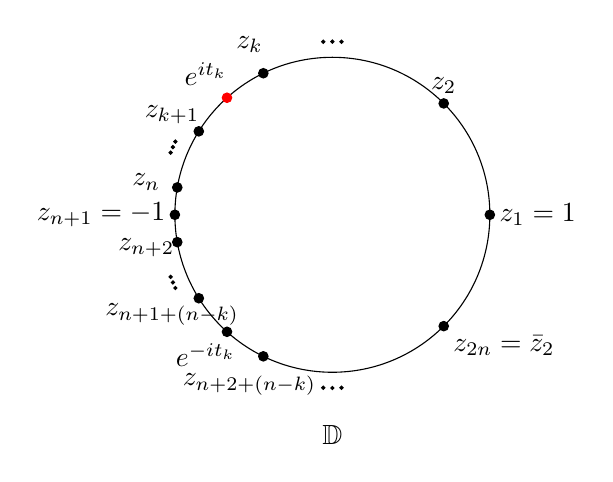
\begin{tikzpicture}[scale=2]
\draw (0,0) circle (1cm);
\foreach \n in {5,...,6}
{
\filldraw(2^\n: -1) circle(0.03cm);
\filldraw(-2^\n: -1) circle(0.03cm);
}
\filldraw(87:1.1) circle(0.01cm);
\filldraw(90:1.1) circle(0.01cm);
\filldraw(93:1.1) circle(0.01cm);
\filldraw(-87:1.1) circle(0.01cm);
\filldraw(-90:1.1) circle(0.01cm);
\filldraw(-93:1.1) circle(0.01cm);
\filldraw(155:1.1) circle(0.01cm);
\filldraw(157:1.1) circle(0.01cm);
\filldraw(159:1.1) circle(0.01cm);
\filldraw(-155:1.1) circle(0.01cm);
\filldraw(-157:1.1) circle(0.01cm);
\filldraw(-159:1.1) circle(0.01cm);

\filldraw(10:-1) circle(0.03cm);
\filldraw(-10:-1) circle(0.03cm);
\filldraw[red] (-48:-1) circle(0.03cm);
\filldraw (48:-1) circle(0.03cm);
\draw (64:-1.2) node{$z_{n+2+(n-k)}$};
\draw (48:-1.2) node{$e^{-it_k}$};
\draw (32:-1.2) node{$z_{n+1+(n-k)}$};
\draw (-64:-1.2) node{$z_{k}$};
\draw (-48:-1.2) node{$e^{it_{k}}$};
\draw (-32:-1.2) node{$z_{k+1}$};
\draw (-10:-1.2) node{$z_n$};
\draw (10:-1.2) node{$z_{n+2}$};
\filldraw(0:1) circle(0.03cm) node[anchor=west]{$z_1 = 1$};
\filldraw(45:1) circle(0.03cm) node[anchor=south]{$z_2$};
\filldraw(-45:1) circle(0.03cm) node[anchor=north west]{$z_{2n} = \bar{z}_2$};
\filldraw(180:1) circle(0.03cm) node[anchor=east]{$z_{n+1} = -1$};
\draw (270:1.4) node{$\D$};

\end{tikzpicture}
\begin{tabular}{c}
$\rightarrow$\\
$f$
\end{tabular}
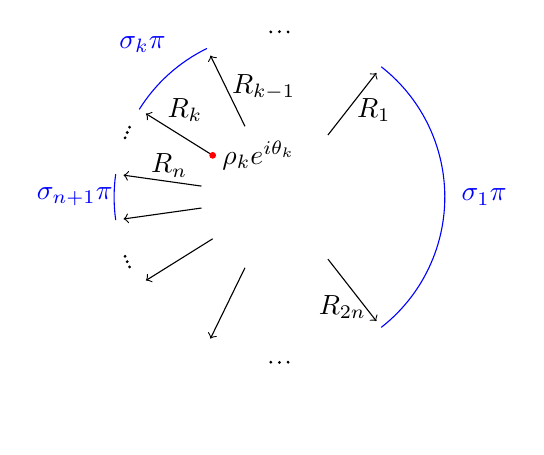
\begin{tikzpicture}[scale=1]
\foreach \n in {5,...,7}
{
\draw[->](2^\n: -1) -- (2^\n: -2);
\draw[->](-2^\n: -1) -- (-2^\n: -2);
}
\draw[->](8:-1) -- (8:-2);
\draw[->](-8:-1)--(-8:-2);
\draw (-0.2,1.4) node{$R_{k-1}$};
\draw (-1.2,1.1) node{$R_k$};
\draw (-1.4,0.4) node{$R_n$};
\draw (1.2,1.1) node{$R_{1}$};
\draw (0.8,-1.4) node{$R_{2n}$};
\filldraw(87:2.1) circle(0.01cm);
\filldraw(90:2.1) circle(0.01cm);
\filldraw(93:2.1) circle(0.01cm);
\filldraw(-87:2.1) circle(0.01cm);
\filldraw(-90:2.1) circle(0.01cm);
\filldraw(-93:2.1) circle(0.01cm);
\filldraw(155:2.1) circle(0.01cm);
\filldraw(157:2.1) circle(0.01cm);
\filldraw(159:2.1) circle(0.01cm);
\filldraw(-155:2.1) circle(0.01cm);
\filldraw(-157:2.1) circle(0.01cm);
\filldraw(-159:2.1) circle(0.01cm);
\filldraw[red] (-32: -1) circle (1pt);
\draw (-32:-1) node[anchor= west]{$\rho_ke^{i\theta_k}$};
\draw[blue] (-64:-2.1) arc (-64:-32:-2.1) ;
\draw[blue] (-48:-2.6) node{$\sigma_k\pi$};
\draw[blue] (128:-2.1) arc (-52:52:2.1) ;
\draw[blue] (0:2.6) node{$\sigma_1\pi$};
\draw[blue] (172:2.1) arc (172:188:2.1);
\draw[blue] (180:2.6) node{$\sigma_{n+1}\pi$};
\draw (270:2.8) node{$\varOmega$};
\end{tikzpicture}

The explicit formula
  \begin{align} \label{f}
  f(z) = z \prod_{j=1}^{2n}(1-\bar{z}_jz)^{-\sigma_j}
  \end{align}
 for $f$ can be given; see \cite[Thm 3.18]{Pom}.


The points $z_k$ correspond to angles $\sigma_k$ dependent on $\rho_k$, the slits' starting moduli.  
The symmetrical setup gives the following equations for $k = 2, 3, ... ,n$.
  $$z_{2n+2-k} = \bar{z}_k.$$
  $$\sigma_{2n+2-k} = \sigma_k.$$
  $$\exp(it_{2n+1-k}) = \exp(-it_k).$$
  $$\rho_{2n+1-k} = \rho_k.$$

If we require that $\rho_k = \rho_j$ for all $j,k$, we can prescribe either $\{z_k\}$ or $\{\sigma_k\}$, but their precise relationship is not obvious.  Denote the arc lengths on the unit circle from $z_k$ to $z_{k+1}$ by
 $$\{\omega_k = |(z_k,z_{k+1})|\},$$
 and it follows that $\omega_k$ is the harmonic measure of the slit $R_k$ in $\varOmega$.
 One natural question is the following.
 \begin{ques} \label{question}
 Does $\{\omega_k\}_1^n$ being monotone imply $\{\sigma_k\}_1^n$ are monotone, and vice versa?
 \end{ques}
 
 We conjecture that the answer is yes, but a proof using classic geometric function theory eludes us.
\vskip10pt


\section{Discretization}


 For convenience let us reflect $\varOmega$ about the imaginary axis and make the slits start on the unit circle. 
 For symmetric slits
\begin{align}
S_k = \{ re^{\pm i \theta_k} :  r \ge 1\} 
\end{align}
satisfying $\theta_0 = 0 < \theta_1 < \theta_2 < ... < \theta_N$ with $(\theta_k - \theta_{k-1}) \leq (\theta_{k+1} - \theta_k)$ for all $k = 1, ... , N-1$, define
\begin{align}
\varOmega = \C \setminus \left( \cup_{k=0}^N S_k \right).
\end{align}
We also denote the channels
\begin{align}
C_k = \{ re^{\pm i \theta} :  r > 1, \theta_k < \theta < \theta_{k+1}\}. 
\end{align}


Following \cite{CS}, for each $\delta > 0$, we define an isoradial graph $\varGamma^{\delta}$ to approximate compact subsets of $\varOmega.$ An \textit{isoradial} graph is planar and consists of faces that are all inscribed in circles of the same radius.  In \cite{CS}, an infinite graph is used, which has the advantage of ensuring a connected boundary exists for any bounded subset.  Here, we use finite $\varGamma^{\delta}$ and eventually describe the boundary explicitly; see Question (\ref{spandrel}) below.

We may assume $\delta^2 = 2\pi/ m$ for some integer $m$.
The vertices along rays spaced by $\Delta \theta = \delta^2$ can extend to radius $1/\delta$, creating graphs that fill $\varOmega$ as $\delta$ tends to 0.  

Specifying the moduli of the vertices,
we begin with $r_0 = 0$.  The isoradial property determines the following recursive formula for $r_j = r_j(\delta)$.
\begin{align} \label{rmoduli}
    r_{j+1} = r_j\cos(\pi/m) + \sqrt{(r_j\cos(\pi/m))^2 - r_j^2 + \delta^2},
\end{align}
which gives the moduli of the circle centers of the graph faces for odd indices, and the moduli of the vertices for even indices.  \textcolor{blue}{ (We stop the recursion once the term in the square root is negative.  It is not obvious that $\# \{r_n\}$ is finite, but it turns out to be so for the simulated values of $\delta$ in question, and in any case we can eschew vertices near the edge without affecting our results.)}

Thus we denote the even indices $\{r_{2n}\}$, and have the vertices
\begin{align}
V(\varGamma^{\delta}) = \{ r_j e^{i\ell\delta^2} :  \ell = 1, ... , m \qquad r_j \in \{r_{2n}\} \}.
\end{align} 
The edges $E(\varGamma^{\delta})$ are between vertex neighbors who share either modulus or argument.


Note again that $r_j \Delta \theta < \delta$, i.e., $r_j < 1/\delta$, is a condition on the maximum $r_j$, which we denote $r^{\delta}_{\text{max}}$.


\begin{figure}[h!]
\centering
\caption{Graph shown in black.  Circle centers are pink.}
\includegraphics[width=8cm]{stargraphq16wC.pdf}
\end{figure}

\begin{figure}[h!]
\centering
\parbox{6cm}{
\caption{Isoradial polar graph with $m = 16$.}
\includegraphics[width=6cm]{stargraphq16.pdf}}
\quad
\begin{minipage}{6cm}
\caption{Isoradial polar graph with $m = 64$.}
\includegraphics[width=6cm]{stargraphq64.pdf}
\end{minipage}
\end{figure}



\newpage

As $\delta \to 0$, $\varOmega$ will be approximated by successively larger and finer grids $\varOmega^{\delta}$ with vertices
\begin{align}
\textcolor{red}{V_{\varOmega^{\delta}} = V(\varGamma^{\delta}) \setminus  S_{\varOmega^{\delta}}}
\end{align}
where the boundary $S_{\varOmega^{\delta}}$ is the closest approximation to the slits $S$, as we describe next.

For every slit tip
$e^{ i \theta_k}$
there exists a nearest set of vertices $\{\gamma_k^{\delta}\} \subset \{V( \varGamma^{\delta}) \}$ such that 
\begin{align}
\gamma_k^{\delta} \to e^{i \theta_k} \text{ as } \delta \to 0,
\end{align}
with a symmetric argument for each $e^{ - i \theta_k}$.
The discrete slit
\begin{align}
(S_k)_{\Omega^{\delta}} = \{ v \in V(\varGamma^{\delta}) : \arg v = \arg \gamma_k^{\delta}, |v| \ge |\gamma_k^{\delta}|\},
\end{align}
and the boundary \textcolor{red}{$\partial \Omega_{\delta} = \partial \Omega_{\varGamma^{\delta}} = \partial \Omega_{\varGamma}^{\delta}$} is a connected set of vertices intersecting
\begin{align}
S_{\Omega^{\delta}} = \cup_{k=0}^N (S_k)_{\Omega^{\delta}}.
\end{align}
Also, the moduli of $\gamma_k^{\delta}$ are the same for all $k$, and approach 1 as $\delta \to 0$.  
Thus, for each $\delta$ we have the disjoint union
\begin{align}
\{v \in V(\varGamma^{\delta}) : |v| = |\gamma_k^{\delta}| \} = \{\gamma_k^{\delta}\} \sqcup \{v^{\delta} \},
\end{align}
with the vertices denoting channel openings
\begin{align}
 \{v^{\delta} \} = \cup_k \{v^{\delta}_{k,\ell}, \quad \ell = 1, ..., n_k^{\delta} \}.
\end{align}
The double index on  $v^{\delta}_{k,\ell}$ will be used below in Brownian motion estimates.  $n_k^{\delta}$ measures the discrete channel width, and 
\begin{align}
n_k^{\delta} \approx (\theta_k - \theta_{k-1})/\delta^2,
\end{align}
with $n_k^{\delta} \leq n_{k+1}^{\delta}$ for all $k$.
For small enough $\delta$, each channel $C_k$ corresponds to interior vertices extending to $r_{\text{max}}^{\delta}$.
(If $\delta$ is not smaller than the $k$th channel width, then $n_k^{\delta} = 0$, and the channel will be excluded from the discrete approximation.)  So the discrete channels are
\begin{align}
(C_k)_{\Omega^{\delta}} = \cup_{\ell = 1}^{n_k} \{ v \in V(\varGamma^{\delta}) : \arg v = \arg v_{k,\ell}^{\delta}, \quad |v_{k,\ell}^{\delta}| \leq |v| < r^{\delta}_{\text{max}}\}.
\end{align}

Our discrete domain $\varOmega_{\varGamma}^{\delta}$ consists of the channels together with the approximation of the unit disk
\begin{align}
\D^{\delta} = \{ v \in V(\varGamma^{\delta}) : |v| \leq |v_{k,\ell}^{\delta}| \approx 1\},
\end{align}
along with a boundary depending on the slits.

I.e., 
\begin{align}
\text{int} \varOmega_{\varGamma}^{\delta} = \left( \D^{\delta} \setminus \{\gamma_k^{\delta} \} \right) \bigcup \cup_k (C_k)_{\Omega^{\delta}},
\end{align}
and 
\begin{align}
\partial \varOmega_{\varGamma}^{\delta} = \{\gamma_k\} \cup \{  (S_k)_{\Omega^{\delta}} : n_k \ne 0 \} \cup \{ v :  \arg v = \arg v_{k,\ell}^{\delta},  |v| = r^{\delta}_{\text{max}} \}.
\end{align}

\begin{figure}[h!]
\centering
\parbox{6cm}{
\caption{Example. Boundary shown in black.}
\label{boundary}
\includegraphics[width=6cm]{stargraphBoundary.pdf}}
\quad
\begin{minipage}{6cm}
\caption{Example. Vertex labelling.}
\includegraphics[width=6cm]{sgbwLabels.png}
\end{minipage}
\end{figure}

\newpage


\textbf{Random walk}

In essence, we employ a discrete version of the famous Kakutani theorem linking Brownian motion with harmonic measure.  The fairly clear intuition is that a random walk has higher probability of landing in a big channel than a small one, thereby achieving the monotonicity conjecture answering Question \ref{question}. We seek to prove that a Brownian traveller on our discrete polar graph with monotone channels maintains a monotonicity of probable location at every step.

As in \cite[p. 1593]{CS}, we define a random walk $RW$ on $\varOmega_{\varGamma}^{\delta}$, where
\begin{align}
RW(t+1) = RW(t) + \xi_{RW(t)}
\end{align} 
and for the neighbors $u_j$ of a vertex $v$ with angles $\theta_j$ 
\begin{align} \label{angles}
\mathbf{P}(\xi_v = u_k - v) = \frac{\tan \theta_k}{\sum_j \tan \theta_j}.
\end{align}
 We will start at the origin, assuming $RW(0) = 0$.  For example, in the first circle
\begin{align}
|u| = r_2^{\delta} \Rightarrow \mathbf{P}(RW(1) = u) = 1/m.
\end{align}
Apart from $0$, all interior vertices have 4 neighbors.
Also, $\theta_u$ is invariant under rotations.  For $B \subset \text{int}\varOmega_{\varGamma}^{\delta}$, we define the discrete harmonic measure $\omega^{\delta}(0;B;\varOmega^{\delta}_{\varGamma})$ to be the probability that the random walk hits $B$ before any other part of the boundary.

Define the channel boundaries as 
\begin{align}
\partial (C_k)_{\Omega^{\delta}} = \{ v \in \partial \varOmega_{\varGamma}^{\delta} : (v,u) \in E(\varGamma^{\delta}), \quad u \in (C_k)_{\Omega^{\delta}} \}.
\end{align}
Our main purpose here is to show that 
\begin{align} \label{channel_monotone}
\omega^{\delta}(0 ; \partial (C_k)_{\Omega^{\delta}}; \varOmega^{\delta}_{\varGamma}) \le \omega^{\delta}(0 ; \partial (C_{k+1})_{\Omega^{\delta}}; \varOmega^{\delta}_{\varGamma}),
\end{align}
implying the harmonic measures of channels are monotone like their widths.  

The probability that $RW$ will land on any vertex $v$ comes from a Markov process encapsulated by a linear map $M$ on the vertices in $\varOmega^{\delta}_{\varGamma}$.  Enumerate all the vertices, and write $M$ as a matrix where $M_{ij}$ is the probability of moving from the $i$th vertex to the $j$th. Let $\mathbf{e_v}$ be the vector with all $0$s except a $1$ in the index corresponding to $v$.  Then
\begin{align}
\mathbf{P}(RW(t) = v) = \mathbf{e_v} \cdot M^t \mathbf{e_0},
\end{align}
where $M^t$ is a product of $t$ copies of $M$, and the dot product extracts the value corresponding to $v$.  Define $M^0$ to be the identity matrix, a square matrix with side length equal to the cardinality of $\varOmega^{\delta}_{\varGamma}$.

 The row corresponding to $v=0$ in the enumeration will be a vector with $m$ nonzero entries with value $1/m$, and the typical interior vertex will correspond to a row with exactly 4 nonzero entries with values around $1/4$ that add to $1$.  The row corresponding to a boundary vertex will have only one nonzero entry, which will be a 1 in the same column as row number.  Evidently, 
 \begin{align}
 \lim_{t \to \infty} \mathbf{e_v} \cdot M^t \mathbf{e_0} 
 \begin{cases}
  &> 0, \quad v \in \partial \varOmega_{\varGamma}^{\delta}\\
  & = 0, \quad v \in \text{int} \varOmega_{\varGamma}^{\delta}
 \end{cases}.
\end{align}

The crux of our argument is the following lemma.  \textcolor{blue}{We need $v^{\delta}_{k,\ell}$ to range over all radii in $\varOmega^{\delta}_{\varGamma}$.  That is, $(k,\ell)$ dictates interior vertex argument, but refers to vertex of arbitrary radius.  Thats not how it was defined above, but assuming it below seems ok for now.}

\begin{lem} \label{lem_interior}
For all $t, k \in \mathbb{N}$, 
\begin{align}\mathbf{P}(RW(t) = v^{\delta}_{k,\ell}) \le \min (\mathbf{P}(RW(t) = v^{\delta}_{k+1,\ell}) , \mathbf{P}(RW(t) =  v^{\delta}_{k+1,n_{k+1}-\ell+1})).
\end{align}
\end{lem}
\begin{proof}
We proceed by induction on $t$.  The base case $t=0$ is clear since all the relevant quantities are 0.  We will write 
\begin{align}
Mvu = \mathbf{P}(RW(t+1) = v \, | \, RW(t) = u)
\end{align}
as a way to refer to entries of the Markov matrix.
For every vertex except the origin, we have the four term Markov process equation
\begin{align}
\mathbf{P}(RW(t+1) = v) &= Mvv_l \mathbf{P}(RW(t) = v_l) 
+ Mvv_r \mathbf{P}(RW(t) = v_r)\\
& + Mvv_u \mathbf{P}(RW(t) = v_u) + Mvv_d \mathbf{P}(RW(t) = v_d).
\end{align}
Here we have denoted the neighbor vertices $v_l, v_r, v_u, v_d$ with a picture of left, right, up, and down in mind.  Rotational invariance and monotonicity of $n_k$ gives
\begin{align} \label{M1}
Mv^{\delta}_{k,\ell}(v^{\delta}_{k,\ell})_a = Mv^{\delta}_{k+1,\ell}(v^{\delta}_{k+1,\ell})_a, \quad a = l, r, u, d,
\end{align}
\textit{except} when $n_{k+1} > n_k = \ell$ and $a = l$, which is when there is a boundary to the left in the $k$th channel but not the $k+1$st.  In this case, $Mv^{\delta}_{k,n_k}(v^{\delta}_{k,n_k})_l = 0$, so the proof below holds.
We also require comparison via intrachannel reflection, which gives
\begin{align}
Mv^{\delta}_{k,\ell}(v^{\delta}_{k,\ell})_r &= Mv^{\delta}_{k+1,n_{k+1}-\ell+1}(v^{\delta}_{k+1,n_{k+1}-\ell+1})_l,\\
Mv^{\delta}_{k,\ell}(v^{\delta}_{k,\ell})_l &= Mv^{\delta}_{k+1,n_{k+1}-\ell+1}(v^{\delta}_{k+1,n_{k+1}-\ell+1})_r.
\end{align}
Then using the inductive assumption and \ref{M1},
\begin{align}
\mathbf{P}(RW(t+1) = v^{\delta}_{k,\ell}) &= Mv^{\delta}_{k,\ell}(v^{\delta}_{k,\ell})_l \mathbf{P}(RW(t) = (v^{\delta}_{k,\ell})_l) \\
&+ Mv^{\delta}_{k,\ell}(v^{\delta}_{k,\ell})_r \mathbf{P}(RW(t) = (v^{\delta}_{k,\ell})_r)\\
& + Mv^{\delta}_{k,\ell}(v^{\delta}_{k,\ell})_u \mathbf{P}(RW(t) = (v^{\delta}_{k,\ell})_u) \\
&+ Mv^{\delta}_{k,\ell}(v^{\delta}_{k,\ell})_d \mathbf{P}(RW(t) = (v^{\delta}_{k,\ell})_d)\\
&\le Mv^{\delta}_{k+1,\ell}(v^{\delta}_{k+1,\ell})_l \mathbf{P}(RW(t) = (v^{\delta}_{k+1,\ell})_l) \\
&+ Mv^{\delta}_{k+1,\ell}(v^{\delta}_{k+1,\ell})_r \mathbf{P}(RW(t) = (v^{\delta}_{k+1,\ell})_r)\\
& + Mv^{\delta}_{k+1,\ell}(v^{\delta}_{k+1,\ell})_u \mathbf{P}(RW(t) = (v^{\delta}_{k+1,\ell})_u) \\
&+ Mv^{\delta}_{k+1,\ell}(v^{\delta}_{k+1,\ell})_d \mathbf{P}(RW(t) = (v^{\delta}_{k+1,\ell})_d)\\
&= \mathbf{P}(RW(t+1) = v^{\delta}_{k+1,\ell}).
\end{align}
The inductive assumption implies that 
\begin{align}
\mathbf{P}(RW(t) = (v^{\delta}_{k,\ell})_l) \le \mathbf{P}(RW(t) = (v^{\delta}_{k+1,n_k+1-\ell})_r),
\end{align}
\textit{except} in the case that $(v^{\delta}_{k,\ell})_l$ is the boundary.  However, in that case $Mv^{\delta}_{k,\ell}(v^{\delta}_{k,\ell})_l$ is 0.  
So we also have
\begin{align}
&\mathbf{P}(RW(t+1) = v^{\delta}_{k,\ell}) = Mv^{\delta}_{k,\ell}(v^{\delta}_{k,\ell})_l \mathbf{P}(RW(t) = (v^{\delta}_{k,\ell})_l) \\
&+ Mv^{\delta}_{k,\ell}(v^{\delta}_{k,\ell})_r \mathbf{P}(RW(t) = (v^{\delta}_{k,\ell})_r)\\
& + Mv^{\delta}_{k,\ell}(v^{\delta}_{k,\ell})_u \mathbf{P}(RW(t) = (v^{\delta}_{k,\ell})_u) \\
&+ Mv^{\delta}_{k,\ell}(v^{\delta}_{k,\ell})_d \mathbf{P}(RW(t) = (v^{\delta}_{k,\ell})_d)\\
&\le Mv^{\delta}_{k+1,n_k+1-\ell}(v^{\delta}_{k+1,n_k+1-\ell})_r \mathbf{P}(RW(t) = (v^{\delta}_{k+1,n_k+1-\ell})_r) \\
&+ Mv^{\delta}_{k+1,n_k+1-\ell}(v^{\delta}_{k+1,n_k+1-\ell})_l \mathbf{P}(RW(t) = (v^{\delta}_{k+1,n_k+1-\ell})_l) \\
& + Mv^{\delta}_{k+1,n_k+1-\ell}(v^{\delta}_{k+1,n_k+1-\ell})_u \mathbf{P}(RW(t) = (v^{\delta}_{k+1,n_k+1-\ell})_u) \\
&+ Mv^{\delta}_{k+1,n_k+1-\ell}(v^{\delta}_{k+1,n_k+1-\ell})_d \mathbf{P}(RW(t) = (v^{\delta}_{k+1,n_k+1-\ell})_d)\\
&= \mathbf{P}(RW(t+1) = v^{\delta}_{k+1,n_k+1-\ell}).
\end{align}
\end{proof}

Having established a monotone property on the interior vertices, we use it to do the same on the boundary slits.


\begin{lem} \label{lem_slit}
For all $t, k \in \mathbb{N}$, 
\begin{align}
\mathbf{P}(RW(t) = \gamma_k^{\delta}) \le \mathbf{P}(RW(t) = \gamma_{k+1}^{\delta}).
\end{align}
\end{lem}
\begin{proof}
Note, for example, that $(\gamma_k^{\delta})_r = v^{\delta}_{k-1,n_{k-1}}$.
The Markov equation is 
\begin{align}
\mathbf{P}(RW(t+1) =  \gamma_k^{\delta}) &= M \gamma_k^{\delta}v^{\delta}_{k-1,n_{k-1}} \mathbf{P}(RW(t) =v^{\delta}_{k-1,n_{k-1}}) \\
&+ M \gamma_k^{\delta}v^{\delta}_{k,1} \mathbf{P}(RW(t) = v^{\delta}_{k,1}) \\
&+ M \gamma_k^{\delta}(\gamma_k^{\delta})_u\mathbf{P}(RW(t) = (\gamma_k^{\delta})_u) \\
&+ M \gamma_k^{\delta}(\gamma_k^{\delta})_d\mathbf{P}(RW(t) = (\gamma_k^{\delta})_d) 
\end{align}
The last two terms are 0 down the slit, but we have to be careful about the tips and the rays inside the unit circle.  It seems to me the inductive assumption takes care of those cases.  And the previous lemma takes care of the first two terms, although we must consider the case $k=0$ where there may be no neighbor vertex to one side, or where, because of symmetry, we need not bother.  Note also Figure \ref{boundary} has an inaccuracy where it shows black vertices in corners which are unreachable, so the formal graph boundary excludes them.
\end{proof}


\textbf{Spandrel}

We use the term \textit{spandrel} in the sense of evolutionary biology, rather than architecture.  A question unimportant to the original goal of research, but curious in its own right, arose while we wrote code in Python and Sagemath to produce images of isoradial graphs.  We were unable to find an algorithm that could generate an infinite graph fitting the starlike appropriate starlike property.  Given $\delta > 0$, we define a \textit{infinite dyadic polar isoradial starlike graph} to be an isoradial graph $\varGamma^{\delta}$ with the following properties:

\begin{enumerate}
\item [(Dyadic)] $v \in V(\varGamma^{\delta})$ implies $\arg v = 2\pi  / 2^n$ for some integer $n$;
\item [(Starlike)] $re^{i\theta} \in V(\varGamma^{\delta})$ implies $r' e^{i\theta} \in V(\varGamma^{\delta})$, where $r' = r \cos(\pi/m) + \sqrt{(r \cos(\pi/m))^2 - r^2 + \delta^2}$;
\item [(Infinite)] for all $r > 0$, there exists $v \in V(\varGamma^{\delta})$ such that $|v| > r$.
\end{enumerate}

\begin{ques} \label{spandrel}
Does an infinite dyadic polar isoradial starlike graph exist?
\end{ques}

We conjecture the answer is no, mostly because we failed to produce one.  If $N(r)$ is the number of vertices on the polar graph with modulus $r$, a successful one would double $N$ at every modulus in a cleverly chosen sequence $\{r_k\}$, which seems to be subject to too many constraints to exist. Below are some images created by our algorithms.

\includegraphics[width=15cm]{iso1.png}

\includegraphics[width=5cm]{iso2.png}

\includegraphics[width=15cm]{iso3.png}

\includegraphics[width=15cm]{stargraph20.pdf}

\newpage

\section{Formal Verification in Lean 4 (2026 Update)}
\sloppy

In 2026, the discrete Kakutani--Markov monotonicity proofs of Section 2 (Lemma \ref{lem_interior}, Lemma \ref{lem_slit}, and the channel harmonic measure monotonicity inequality (\ref{channel_monotone})), the analytic starlike and Herglotz--Pommerenke theory of Section 1 (\ref{f}), the exact trigonometric discriminant identity for (\ref{rmoduli}), and the $\eps$-$\delta$ continuum reduction from discrete to continuum channel monotonicity were formalized and machine-verified in the \textbf{Lean 4} interactive theorem prover.

\subsection*{Public Lean 4 Repositories}
\begin{itemize}
\item \textbf{Slit Harmonic Measure \& Isoradial Discretization (\texttt{SlitHarmonicMeasure.lean}):}
\begin{center}
{\footnotesize \url{https://github.com/aanderson3456/MyLean4Code/blob/main/ComplexAnalysis/SlitHarmonicMeasure.lean}}
\end{center}
\item \textbf{Polar-Angle Starlike Domains \& Herglotz--Pommerenke Theory (\texttt{Sarason/Chapter3.lean}):}
\begin{center}
{\footnotesize \url{https://github.com/aanderson3456/MyLean4Code/blob/main/ComplexAnalysis/Sarason/Chapter3.lean}}
\end{center}
\end{itemize}

\subsection*{1. Real-Valued Formalization of Lemma \ref{lem_interior} (Interior Channel Monotonicity)}

In Sections 8--10 of \texttt{SlitHarmonicMeasure.lean}, the 4-neighbor Markov transition operator (\ref{angles}) with Chelkak--Smirnov tangent weights $\texttt{isoradialTangentWeight}(\theta_k, \theta_{\text{sum}}) = \tan\theta_k / \theta_{\text{sum}}$ is formalized over $\R$ via the bilinear transition step
\[
\texttt{markovFourTermStep\_R}(m_l, m_r, m_u, m_d, p_l, p_r, p_u, p_d)
= m_l p_l + m_r p_r + m_u p_u + m_d p_d.
\]
To capture both the rotational symmetry (\ref{M1}) and the boundary absorption exception when $n_{k+1} > n_k = \ell$ and $a = l$ (where the left neighbor of $v^{\delta}_{k,n_k}$ lies on the absorbing slit boundary $(S_k)_{\Omega^{\delta}}$, forcing $m_{l,k} = 0 \le m_{l,k+1}$, whereas $m_{l,k} = m_{l,k+1}$ at all interior positions), the weight hypothesis is unified into $0 \le m_{l,k} \le m_{l,k+1}$. Similarly, under the intrachannel reflection $\ell \mapsto n_{k+1} - \ell + 1$, the left and right transition weights swap ($0 \le m_{l,k} \le m_{r,\text{refl}}$). The theorems \texttt{lemma\_2\_1\_direct\_step\_R}, \texttt{lemma\_2\_1\_reflected\_step\_R}, and the full time-induction theorem \texttt{lemma\_2\_1\_full\_induction\_R} machine-verify Lemma \ref{lem_interior} over $\R$ for all $t \in \N$:

{\small
\begin{verbatim}
def markovFourTermStep_R (ml mr mu md pl pr pu pd : R) : R :=
  ml * pl + mr * pr + mu * pu + md * pd

theorem lemma_2_1_full_induction_R (W : CoupledChannelWalk_R) (t : N) :
    probChannelK_R W t <=
      min (probChannelDirect_R W t) (probChannelRefl_R W t)
\end{verbatim}
}
Starting from the base case $\mathbf{P}(RW(0) = v^{\delta}_{k,\ell}) = 0$ (since $RW(0) = 0$ at the origin while channel vertices satisfy $|v| \ge |\gamma^{\delta}_k| > 0$), \texttt{lemma\_2\_1\_full\_induction\_R} establishes that for every time step $t \in \N$,
\begin{align*}
\mathbf{P}(RW(t) = v^{\delta}_{k,\ell}) &\le \min\bigl(\mathbf{P}(RW(t) = v^{\delta}_{k+1,\ell}),\, \mathbf{P}(RW(t) = v^{\delta}_{k+1,n_{k+1}-\ell+1})\bigr).
\end{align*}

\subsection*{2. Real-Valued Formalization of Lemma \ref{lem_slit} \& Equation (\ref{channel_monotone})}

Specializing Lemma \ref{lem_interior} to $\ell = 1$ yields both neighbor inequalities required at the slit vertices $\gamma^{\delta}_k$ and $\gamma^{\delta}_{k+1}$:
\begin{enumerate}
\item From the intrachannel-reflected bound at $\ell = 1$ on channels $k-1$ and $k$:
\[
\mathbf{P}(RW(t) = v^{\delta}_{k-1, n_{k-1}}) \le \mathbf{P}(RW(t) = v^{\delta}_{k, n_k}).
\]
\item From the direct (right-aligned) bound at $\ell = 1$ on channels $k$ and $k+1$:
\[
\mathbf{P}(RW(t) = v^{\delta}_{k, 1}) \le \mathbf{P}(RW(t) = v^{\delta}_{k+1, 1}).
\]
\end{enumerate}
Feeding these two inequalities into \texttt{lemma\_2\_2\_slit\_boundary\_monotonicity\_R} verifies Lemma \ref{lem_slit} over $\R$:
\[
\mathbf{P}(RW(t+1) = \gamma^{\delta}_k) \le \mathbf{P}(RW(t+1) = \gamma^{\delta}_{k+1}).
\]
For the discrete channel widths $n_k^{\delta} = \lfloor \Delta\theta_k / \delta^2 \rfloor_{\N}$ (\texttt{discreteChannelWidth\_delta}), the theorem \texttt{discreteChannelWidth\_delta\_monotone} proves that monotone continuum channel opening angles $\Delta\theta_k \le \Delta\theta_{k+1}$ imply $n_k^{\delta} \le n_{k+1}^{\delta}$ for every mesh parameter $\delta \in \R$. Summing the non-negative absorbed boundary hitting probabilities over $\ell \in \{1, \dots, n_k^{\delta}\} \subseteq \{1, \dots, n_{k+1}^{\delta}\}$ via \texttt{discrete\_channel\_harmonic\_measure\_monotone\_R} establishes Equation (\ref{channel_monotone}) over $\R$:
\[
\omega^{\delta}(0 ; \partial (C_k)_{\Omega^{\delta}}; \varOmega^{\delta}_{\varGamma})
= \sum_{\ell=1}^{n_k^{\delta}} p_{k,\ell}
\le \sum_{\ell=1}^{n_{k+1}^{\delta}} p_{k+1,\ell}
= \omega^{\delta}(0 ; \partial (C_{k+1})_{\Omega^{\delta}}; \varOmega^{\delta}_{\varGamma}).
\]

\subsection*{3. Polar-Angle Starlike Theory \& Herglotz--Pommerenke Slit Maps (\texttt{\_eps})}

In \texttt{Sarason/Chapter3.lean} (\S III.13) and \texttt{SlitHarmonicMeasure.lean} (\S 8--\S 9), the analytic framework of Section 1 is formalized in terms of polar coordinates $\texttt{polarPoint}(r,\theta) = r(\cos\theta + i\sin\theta)$ and Weierstrass $\eps$-$\delta$ complex differentiability (\texttt{HasDerivAt\_eps}, \texttt{HolomorphicOn\_eps}):
\begin{enumerate}
\item \textbf{Starlike Slit Domains (\texttt{slitDomain\_Omega\_isStarlike\_theta}):}
Proves that the slitted domain $\varOmega = \C \setminus \bigcup_{k=0}^N S_k$ is starlike with respect to the origin in the polar-angle sense (\texttt{IsStarlikeDomain\_theta}), i.e., if $\texttt{polarPoint}(r,\theta) \in \varOmega$ and $0 \le t \le 1$, then $\texttt{polarPoint}(tr,\theta) \in \varOmega$.
\item \textbf{Logarithmic Derivative Characterization (\texttt{isStarlikeOnDisk\_theta\_eps\_iff\_logDeriv\_eps}):}
Proves $\frac{\partial}{\partial\theta}\arg f(re^{i\theta}) = \re\!\left(\frac{zf'(z)}{f(z)}\right)$, establishing that an analytic map $f$ on $\D$ is starlike in $\theta$ if and only if $\re\!\left(\frac{zf'(z)}{f(z)}\right) > 0$ on $\D \setminus \{0\}$.
\item \textbf{Herglotz--Pommerenke Logarithmic Derivative (\texttt{pommerenkeLogDeriv}):}
For the slit Riemann map (\ref{f}), the logarithmic derivative
\[
\frac{z f'(z)}{f(z)} = \sum_{j=1}^{2n} \frac{\sigma_j}{2}\frac{z_j + z}{z_j - z}
\]
is proved to be holomorphic on $\D$ in the Weierstrass $\eps$-$\delta$ sense (\texttt{pommerenkeLogDeriv\_holomorphicOn\_eps}), to have strictly positive real part on $\D$ (\texttt{pommerenkeLogDeriv\_re\_pos\_on\_disk}), to have vanishing real part on $\partial\D \setminus \{z_j\}$ (\texttt{pommerenkeLogDeriv\_re\_zero\_on\_circle}), and to satisfy the exact boundary cotangent identity on $\partial\D$ (\texttt{pommerenkeLogDeriv\_unitCircle\_eq}):
\[
\sum_{j=1}^{2n} \frac{\sigma_j}{2}\frac{e^{i\phi_j} + e^{it}}{e^{i\phi_j} - e^{it}}
= i \sum_{j=1}^{2n} \frac{\sigma_j}{2}\frac{\sin(t - \phi_j)}{1 - \cos(t - \phi_j)}.
\]
In particular, at a slit-tip preimage $e^{it_k} \in \partial\D$, $f'(e^{it_k}) = 0$ if and only if the boundary cotangent sum vanishes (\texttt{pommerenkeLogDeriv\_eq\_zero\_on\_circle\_iff\_cotangentSum\_eq\_zero}).
\end{enumerate}

\subsection*{4. Chelkak--Smirnov Discrete Mean Value Theorem, Laplacian Consistency with \texttt{IsRealHarmonicOn\_eps}, and Analytic--Discrete Proof Transfer}

In Section 11 of \texttt{SlitHarmonicMeasure.lean}, the internal discrete complex analysis of Chelkak and Smirnov \cite[Secs.~2.1--2.2 \& Sec.~3]{CS} linking the discrete random walk on $\varGamma^{\delta}$ to the continuum Mean Value Property and Laplacian is formalized:
\begin{enumerate}
\item \textbf{Dual-Circle Telescoping \& Exact First-Order Cancellation (\texttt{IsoradialVertexStar}, \texttt{isoradialStar\_weighted\_displacement\_sum\_eq\_zero}):}
At each interior vertex $v \in \C$, every primal edge $u_k - v$ is orthogonal to the dual circumcenter chord $w_k - w_{k-1}$ ($|w_k - v| = \delta$) via $(\tan\theta_k)(u_k - v) = -i(w_k - w_{k-1})$. Summing around the closed dual cycle $\sum_{k=1}^d (w_k - w_{k-1}) = 0$ yields
\[
\sum_{k=1}^d \tan\theta_k\,(u_k - v) = 0, \qquad
\sum_{k=1}^d \tan\theta_k\,(u_k - v).\re = 0, \qquad
\sum_{k=1}^d \tan\theta_k\,(u_k - v).\im = 0.
\]
\item \textbf{Discrete Laplacian $\Delta^{\delta}$ $\iff$ Discrete Mean Value Theorem (\texttt{isDiscreteHarmonicAt\_iff\_meanValueProperty}, \texttt{affine\_isDiscreteHarmonicAt}):}
For the Chelkak--Smirnov discrete Laplacian $(\Delta^{\delta} H)(v) = \frac{1}{\mu_{\varGamma}(v)}\sum_{k=1}^d \tan\theta_k\,(H(u_k) - H(v))$ with $\mu_{\varGamma}(v) = \frac{1}{4}\sum_{k=1}^d \tan\theta_k\,\|u_k - v\|^2$, the theorem \texttt{isDiscreteHarmonicAt\_iff\_meanValueProperty} proves
\[
(\Delta^{\delta} H)(v) = 0 \iff H(v) = \sum_{k=1}^d \left(\frac{\tan\theta_k}{\sum_{j=1}^d \tan\theta_j}\right) H(u_k) = (M^{\delta} H)(v).
\]
In particular, all real affine functions $H(z) = a\re z + b\im z + c$ are exactly discrete harmonic (\texttt{affine\_isDiscreteHarmonicAt}).
\item \textbf{Second-Order Laplacian Consistency with \texttt{IsRealHarmonicOn\_eps} (\texttt{isoradialDiscreteLaplacian\_secondOrderTaylorAt}, \texttt{isRealHarmonicOn\_eps\_imp\_discreteMeanValue\_and\_remainder}):}
On any quadratically balanced star ($\sum_{k=1}^d \tan\theta_k\,(u_k - v)^2 = 0$), the discrete Laplacian of a second-order Taylor polynomial $T_2(z)$ at $v$ equals the exact continuum Laplacian $h_{xx} + h_{yy}$. When $h$ satisfies \texttt{IsRealHarmonicOn\_eps} ($h_{xx} + h_{yy} = 0$), its second-order Taylor jet $T_2$ satisfies the exact Discrete Mean Value Property $T_2(v) = (M^{\delta} T_2)(v)$ and $(\Delta^{\delta} h)(v) = \Delta^{\delta}(h - T_2)(v) \to 0$ as $\delta \to 0$ (\texttt{isRealHarmonicOn\_eps\_imp\_discreteLaplacian\_tendsto\_zero\_eps}).
\item \textbf{Discrete Maximum Principle \& Analytic--Discrete Proof Transfer (\texttt{isoradial\_local\_maximum\_principle}, \texttt{chelkak\_smirnov\_convergence\_hasLimitAt\_eps}, \texttt{chelkak\_smirnov\_analytic\_discrete\_transfer\_eps}):}
Proves the local discrete maximum principle, establishes Weierstrass \texttt{HasLimitAt\_eps} convergence $H^{\delta}(v) \to h(v)$ from the boundary and Laplacian consistency errors, and chains with \texttt{analytic\_truncated\_channel\_monotone\_of\_hasLimitAt\_eps} ($\delta \to 0$) and \texttt{analytic\_monotone\_channel\_of\_hasLimitAtInf\_eps} ($\|w\| \to \infty$) to transfer discrete random-walk monotonicity to the continuum (\texttt{monotoneChannelStatement\_eps\_proven}).
\end{enumerate}

\medskip
\noindent\textbf{Unconditional vs.\ Conditional Status:}
\begin{itemize}
\item \textbf{Unconditionally Verified in Lean 4:}
The 4-term Markov transition inequalities (Lemmas \ref{lem_interior} and \ref{lem_slit}) under coupled neighbor dominance (\texttt{CoupledChannelWalk\_R}), the monotonicity of discrete channel widths $n_k^{\delta} \le n_{k+1}^{\delta}$ and discrete channel harmonic measures (\ref{channel_monotone}) over $\R$, the trigonometric identity $(r_j\cos(\pi/m))^2 - r_j^2 + \delta^2 = \delta^2 - r_j^2\sin^2(\pi/m)$ (\texttt{isoradial\_discriminant\_identity}), the starlike and Herglotz--Pommerenke complex analysis theorems in \texttt{Sarason/Chapter3.lean}, the Chelkak--Smirnov dual-circle telescoping, Discrete Mean Value Theorem, second-order Laplacian consistency with \texttt{IsRealHarmonicOn\_eps}, local discrete maximum principle, and the $\eps$-$\delta$ analytic--discrete proof transfer theorems (\texttt{chelkak\_smirnov\_analytic\_discrete\_transfer\_eps}, \texttt{analytic\_truncated\_channel\_monotone\_of\_hasLimitAt\_eps}, and \texttt{analytic\_monotone\_channel\_of\_hasLimitAtInf\_eps}) are all proved unconditionally with zero axioms or \texttt{sorry}s.
\item \textbf{Remaining Conditional Hypotheses for Question \ref{question} and Question \ref{spandrel}:}
A complete unconditional resolution of Question \ref{question} from first principles still requires: (i) discharging the global neighbor coupling across the unslitted inner disk $|v| < 1$ where rays $\arg \gamma_k^{\delta}$ are interior rather than absorbing, (ii) discharging the global green-function / Beurling--Nevanlinna truncation error estimates on $\varOmega_R$, and (iii) bridging channel monotonicity $\omega(0; \partial C_k; \varOmega) \le \omega(0; \partial C_{k+1}; \varOmega)$ (which pairs the upper bank of slit $k$ with the lower bank of slit $k+1$) to single-slit monotonicity $\omega_k = \omega(0; R_k^-; \varOmega) + \omega(0; R_k^+; \varOmega)$ and its converse under equal starting moduli $\rho_k = \rho_j$. Likewise, Question \ref{spandrel} (\texttt{Question\_2\_3\_Spandrel}) remains an open problem.
\end{itemize}

\begin{thebibliography}{99}

\bibitem{CS} D.~Chelkak (\url{https://www-personal.umich.edu/~chelkak/}) and S.~Smirnov (\url{http://www.unige.ch/~smirnov/}), {\em Discrete complex analysis on isoradial graphs}, Adv.\ Math.\ \textbf{228} (2011), no.~3, 1590--1630 (\href{https://doi.org/10.1016/j.aim.2011.06.025}{doi:10.1016/j.aim.2011.06.025}, \href{https://arxiv.org/abs/0810.2188}{arXiv:0810.2188}).


\bibitem{Pom} Ch.~Pommerenke, {\em Boundary Behavior of Conformal Maps\/},
Springer-Verlag 1992.

\end{thebibliography}
 \end{document}

%%%%%%%%%%%%%%%%%%%%%%%%%
